
\section{Results}

\subsection{Predicting Performance on the MED Dataset}

Figure \ref{fig:blb} displays the EERs of the video detection system on both the Kindred and MED data sets along with the BLB predicted standard deviations for each event. 
The average EERs for the Kindred and MED datasets are 36.1\% and 34.9\%, respectively. 
The average predicted standard deviation is 7.1\% and the average difference between event EERs for the Kindred and MED dataset in terms of predicted standard deviations for that event is .60. 
Interestingly, events 6-15 have an average number of 123.9 positives while events 21-30 have an average of 24 positives in the MED test set and this results in a significantly lower standard deviation of 4.2\% versus 9.9\% for the former. 
This indicates that high numbers of test positives may lead to more refined performance prediction estimates.  

Although not all event EERs fall within one event standard deviation of each other, with the largest gap coming from event 6 with a 1.77 standard deviation gap, the performance on the MED dataset is reasonably bounded by the BLB's predictions. 
This suggests that despite high acoustic variability and little structure, classification performance on consumer-produced multimedia files can be consistently predicted. 

\begin{figure}[ht]
\centering
\subfigure[Events 6-15]{
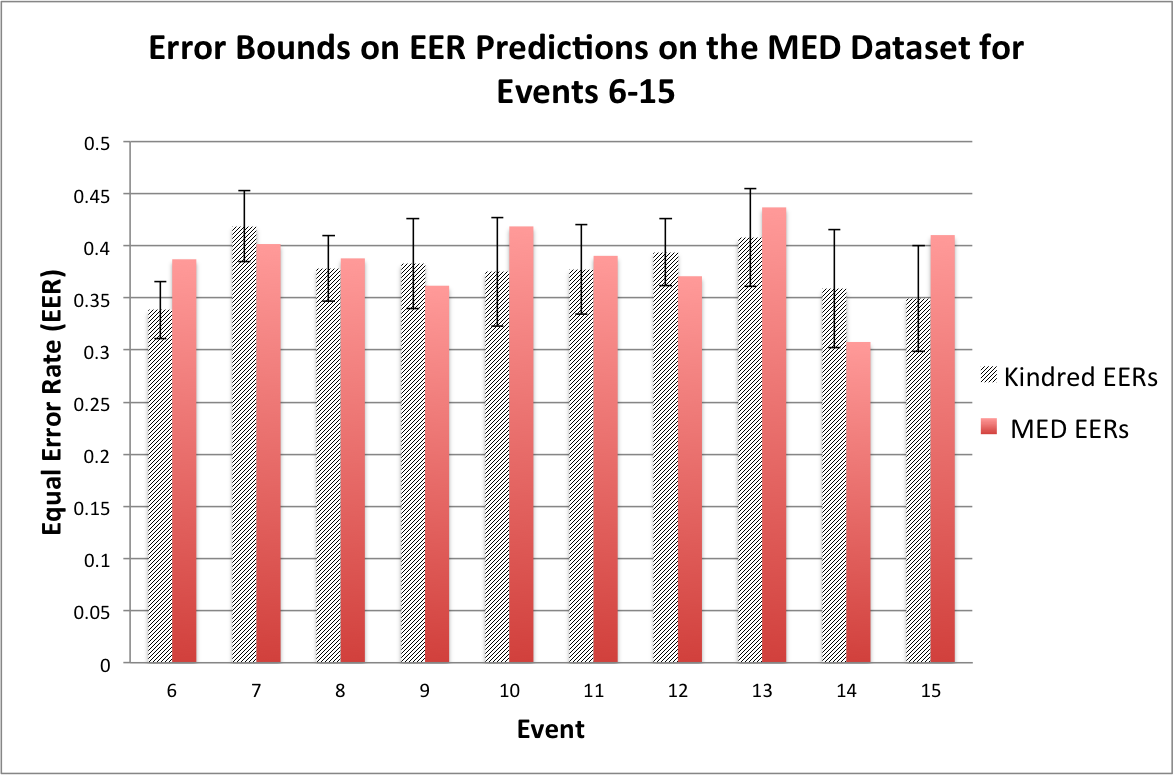
\epsfig{file=figures/errorbounds6-15.png, height=2.0 in, width=3.3in}
\label{fig:blb1}}
\subfigure[Events 21-30]{
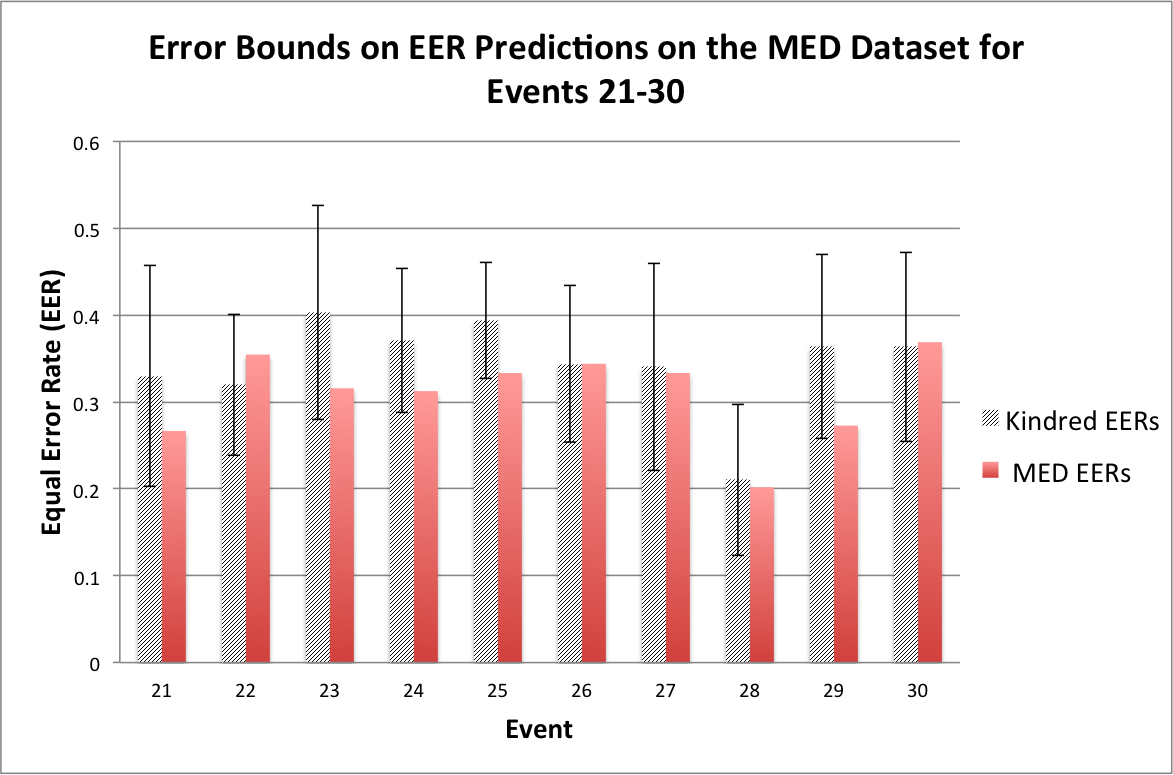
\epsfig{file=figures/errorbounds21-30.png, height=2.0 in, width=3.3in}
\label{fig:blb2}}
\caption{The performance of the video detection system on the Kindred and MED datasets. 
 The error bars display the BLB standard deviations that estimate the variance on the MED dataset from the performance on the Kindred dataset.}
\label{fig:blb}
\end{figure}


\subsection{Comparison to Na\"ive Python}
\begin{figure}
\centering
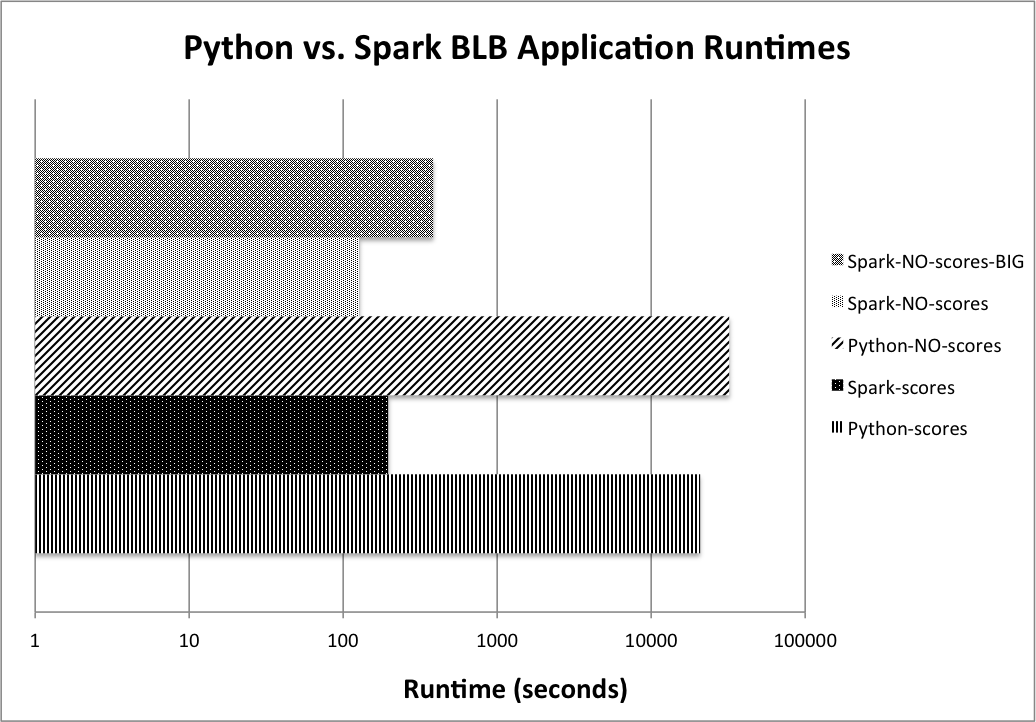
\epsfig{file=figures/pythoncompare.png, height=1.9in, width=3.3in}
\caption{Comparison of runtimes of native Python and generated Spark code. The Spark code, finishing in less than 7 minutes achieves more than a 2 order of magnitude speedup over the 5+ hour Python times. The largest bar is the extrapolated runtime of Python on the BLB application that computes the scores with 100 times more bootstraps to compute than it we test with.}
\label{fig:python}
\end{figure}
 
 As seen in Figure \ref{fig:python}, the Spark code achieves more than a two order of magnitude speedup over the Python code, for both BLB applications tested. The Python code requires an average of 20681 seconds (5.74 hours) and 32142 seconds (8.93 hours) to run when given scores and when not, respectively, whereas the Spark code requires an average of 197.14 seconds (3.29 minutes) and 127.74 seconds (2.13 minutes) to run when given scores and when not, respectively. 
 We can extrapolate runtimes for the BLB application that computes the scores for larger applications. Increasing the number of subsamples and bootstraps up to 20 and 50, respectively, results in 100 (10*10) times more estimates on bootstraps that need to be computed. A 100-fold increase in runtime would amount to a total runtime of 892 hours, likely longer than a researcher's patience would last. 

However, the generated Spark code completes in under 7 minutes, nearly 4 orders of magnitude better than the extrapolated Python runtime. The generated code performs better here relatively since the increased computational load supports a far greater degree of parallelism, whereas on the smaller computation with only 2 subsamples and 5 bootstraps, the need for only 10 bootstrap estimates severly caps the maximum paralellism. This trend of the generated code increasingly outperforming the Python code as the bootstrap computations needed and input data size increase would presumably remain true with more taxing applications since the generated code can simply run on more and more nodes to accomodate the higher demand. 



